\documentclass[acmtog, review, anonymous]{acmart}

\usepackage{booktabs} % For formal tables

% TOG prefers author-name bib system with square brackets
\citestyle{acmauthoryear}
\setcitestyle{square}


\usepackage[ruled]{algorithm2e} % For algorithms
\renewcommand{\algorithmcfname}{ALGORITHM}
\SetAlFnt{\small}
\SetAlCapFnt{\small}
\SetAlCapNameFnt{\small}
\SetAlCapHSkip{0pt}
\IncMargin{-\parindent}

% Metadata Information
\acmJournal{TOG}
% \acmVolume{9}
% \acmNumber{4}
% \acmArticle{39}
% \acmYear{2010}
% \acmMonth{3}

% Copyright
%\setcopyright{acmcopyright}
%\setcopyright{acmlicensed}
%\setcopyright{rightsretained}
%\setcopyright{usgov}
% \setcopyright{usgovmixed}
%\setcopyright{cagov}
%\setcopyright{cagovmixed}

% DOI
% \acmDOI{0000001.0000001_2}

% Paper history
% \received{February 2007}
% \received{March 2009}
% \received[final version]{June 2009}
% \received[accepted]{July 2009}


% Document starts
\begin{document}
% Title portion
\title{OptCuts: Joint Optimization for Seam Placement and Parameterization of 3D Surfaces} 

\author{Minchen Li}
% \orcid{1234-5678-9012-3456}
% \affiliation{%
%   \institution{College of William and Mary}
%   \streetaddress{104 Jamestown Rd}
%   \city{Williamsburg}
%   \state{VA}
%   \postcode{23185}
%   \country{USA}}
\email{minchernl@gmail.com}
% \author{Valerie B\'eranger}
% \affiliation{%
%   \institution{Inria Paris-Rocquencourt}
%   \city{Rocquencourt}
%   \country{France}
% }
% \email{beranger@inria.fr}
% \author{Aparna Patel} 
% \affiliation{%
%  \institution{Rajiv Gandhi University}
%  \streetaddress{Rono-Hills}
%  \city{Doimukh} 
%  \state{Arunachal Pradesh}
%  \country{India}}
% \email{aprna_patel@rguhs.ac.in}
% \author{Huifen Chan}
% \affiliation{%
%   \institution{Tsinghua University}
%   \streetaddress{30 Shuangqing Rd}
%   \city{Haidian Qu} 
%   \state{Beijing Shi}
%   \country{China}
% }
% \email{chan0345@tsinghua.edu.cn}
% \author{Ting Yan}
% \affiliation{%
%   \institution{Eaton Innovation Center}
%   \city{Prague}
%   \country{Czech Republic}}
% \email{yanting02@gmail.com}
% \author{Tian He}
% \affiliation{%
%   \institution{University of Virginia}
%   \department{School of Engineering}
%   \city{Charlottesville}
%   \state{VA}
%   \postcode{22903}
%   \country{USA}
% }
% \affiliation{%
%   \institution{University of Minnesota}
%   \country{USA}}
% \email{tinghe@uva.edu}
% \author{Chengdu Huang}
% \author{John A. Stankovic}
% \author{Tarek F. Abdelzaher}
% \affiliation{%
%   \institution{University of Virginia}
%   \department{School of Engineering}
%   \city{Charlottesville}
%   \state{VA}
%   \postcode{22903}
%   \country{USA}
% }

\renewcommand\shortauthors{Li, M. et al}

\begin{abstract}
Parameterizing 3D surfaces to the 2D plane with low mapping distortion is a critical problem in computer graphics with many applications including texture mapping, remeshing, and detail transfer. 
In most practical cases, it is not possible to map 3D surfaces to the 2D plane without introducing discontinuities (seams) and distortion. Most existing techniques follow a two step process - first placing seams and then minimizing distortion - that usually leads to suboptimal results. 
In this paper, we attack seam placement and parameterization jointly in a single alternating optimization framework, where seams are optimally and progressively introduced \textcolor{red}{or removed} (in topology steps) in between distortion minimization (in descent steps). A linear combination of symmetric Dirichlet energy and seam length are taken as our objective, of which the stationary w.r.t. both UV topology and UV coordinates are guaranteed to be reached within a bounded number of alternating iterations per objective, input model, and initial embedding.

Specifically, in descent steps, we minimize symmetric Dirichlet energy using projected Newton method given the current UV topology. In topology steps, we search for a nearby UV topology that locally decrease the objective the most by querying a filtered set of basic topological operations. To be appropriately aggressive on searching in the topological space, \textcolor{red}{we develop an analogous line search method as in continuous settings}.
\textcolor{red}{Since in application scenarios, an upper bound for distortion or seam length is more intuitive than picking a balancing factor, we also provide a constrained optimization view of this broader problem that seeks stationary w.r.t. both primal (distortion and seams) and dual (balancing factor) variables subject to user specified upper bounds.}

Our method automatically produces both visually pleasing and high quality UV maps with low mapping distortion and an optimally sparse set of seams without any user assistance. \textcolor{red}{We also show that given a UV configuration by other methods, our method can improve the distortion and seam placement}, and our framework has the potential to handle bijectivity, seamlessness, and user preferences jointly within it as well.
\end{abstract}


%
% The code below should be generated by the tool at
% http://dl.acm.org/ccs.cfm
% Please copy and paste the code instead of the example below. 
%
\begin{CCSXML}
<ccs2012>
	<concept>
		<concept_id>10010147.10010371.10010396.10010398</concept_id>
		<concept_desc>Computing methodologies~Mesh geometry models</concept_desc>
		<concept_significance>500</concept_significance>
	</concept>
</ccs2012>
\end{CCSXML}

\ccsdesc[500]{Computing methodologies~Mesh geometry models}

%
% End generated code
%


\keywords{geometry processing, mesh parameterization, seam placement, numerical optimization, ...}



\maketitle

% !TeX root = OptCuts.tex

\section{Introduction}
% context
Mapping three-dimensional meshes to the plane is a fundamental task in computer graphics.  Planar images are commonly used to store reflectance functions, normals, and displacements
for the mesh, providing a domain for painting, synthesizing, and manipulating texture and geometric details. 
%Mesh parameterization is a critical task in computer graphics, with applications including texture mapping, remeshing, and detail transfer.  
%\vova{I removed non-texture apps for now, because I'm not sure if our formulation is as easy to motivate for remeshing and detail transfer.}
At its core, parameterization seeks to find a mapping from a surface---typically represented as a triangle mesh---into the plane.  To do so, parameterization tools must cope with intertwined challenges in topology and geometry:  a high-quality parameterization must cut a surface into simple %disk-shape 
patches so that each can be mapped to the plane with a reasonably small level of distortion.

Given its broad applicability, it comes as no surprise that parameterization has long been a focus of research in geometry processing.  Algorithms in this domain focus on two key aspects of the problem.  Particularly well-studied are \emph{geometric} techniques that assume a surface has already been cut into disk-topology pieces that each need to be mapped into the plane while maintaining fixed connectivity; at this point, parameterization becomes a real-valued optimization problem that seeks to minimize changes in angles and areas while maintaining local or global injectivity. Complementing these techniques, \emph{topological} algorithms find reasonable seams partitioning a surface into individual pieces that can be parameterized.  

With a few notable exceptions, previous works treat seam placement and fixed-topology mapping as separate steps in the parameterization pipeline.  This is a key drawback, as seam placement and complexity have strong bearing on the best \emph{possible} geometric parameterization of each patch.  Coupling geometry and topology, however, requires navigating between two extremes: a zero-distortion but topologically complex parameterization maps every triangle into the plane independently, while a high-distortion but topologically simple mapping might only require puncturing a few points in the input surface.
%
%\vova{not sure if we need to discuss the two extremes. I also moved some prior work discussion here.} % justin kind of likes this sentence so he decided to comment out Vova's comment :-)
%
Most previous techniques rely on heuristics for seam placement, such as computing minimal spanning tree that traverses all points with high curvature~\cite{Sheffer2002Seamster}, cutting between points of maximal distortion~\cite{Gu2002Geometry}, or greedily introducing seams during iterative flattening~\cite{BoundedDistortParam:2002}. In contrast to these methods, we propose a joint optimization framework, where discrete and continuous steps minimize the same global objective. 

% task and object    
Our parameterization algorithm, {\em OptCuts}, %couples topology and geometry. OptCuts %<--- already said this
is a jointly discrete-continuous optimization that progressively updates seam placements in between distortion minimizations to search for a locally optimal UV map satisfying an arbitrary, user-provided, distortion bound. 
%
We measure the trade-off between topology and geometry by balancing a distortion measure of choice, e.g.\ the symmetric Dirichlet energy~\cite{Smith2015Bijective}, with normalized seam length, reaching a parameterization that is near-stationary with respect to both seam placement and coordinate positions. % within a bounded number of iterations. % Justin removed --- I'm not sure this is a feature worth selling unless the bound is favorable
%\minchen{[NOTE] (Here stationary w.r.t. UV topology is only in the approximation sense, because there might still be basic topological operations that could decrease the objective but end up not chosen because it is filtered out or its locally evaluated energy decrease is not the largest one.)}

% self-weighting
%Although we acquire adaptivity to various inputs by normalizing the energy, %<-- not sure what this means
Measuring a balance between distortion and seam length has previously required a choice of a relative scaling factor between these two objectives.  From a practical perspective, it is difficult for users to choose such a coefficient. %trading off between the two. 
%Likewise, i
In practice, for high-quality solutions this balancing factor must be %somehow 
manually updated---often by user intervention during the parametrization process\ \cite{Poranne2017Autocuts}. We instead construct our coupled seam and mapping optimization as a \emph{constrained} problem. We propose to find locally minimal seam lengths for any user-set distortion bound. Treating distortion bounds as a hard inequality constraint guarantees a pre-specified level of geometric quality, while simultaneously enabling the exploration of optimal seams satisfying the bound. %In turn, o %<--- not sure what ``in turn'' means in this context
In turn, as we show below our balancing scaling factor falls directly from our model problem as the \emph{Lagrange multiplier} of the distortion bound and is thus adaptively updated directly by seeking optimality during the course of minimization process.  %directly by our optimization method.
%(Section~\ref{sec:self_weighting}).

% challenge
%Another advantage of our method is that our optimization is combinatorial, 
%
%In contrast to previous work building up a parameterization from disconnected triangle soup~\cite{Poranne2017Autocuts},  or by cutting between points of maximal predicted distortion~\cite{Gu2002Geometry,Sheffer2002Seamster}, 
%
Instead of building up a parameterization from disconnected triangle soup~\cite{Poranne2017Autocuts}, our constrained optimization method minimizes seams combinatorially, directly extending real-valued distortion minimization to the regime where seams can be incrementally introduced by cutting and removed by merging. Distortion is typically reduced by line search in UV coordinate space; we now accompany this by introducing a secondary search procedure in ``topology space'': we alternate between reducing distortion on vertex position and introducing topology changes with respect to the first-order reduction they generate in our objective formed by the local weighted sum of distortion and seam length terms. %in each topology search iteration we first find a search direction that locally decrease the objective the most (in topology step, Section~\ref{sec:topologyStep}); and then we conduct a newly derived forward-tracking line search scheme alternated with distortion minimization iterations to decide the step-size (in smooth descent step, Section~\ref{sec:descentStep}).% too much detail for intro
%\vova{Maybe the relationship to seam placement heuristics can be discussed earlier...}


% experiments
%\justin{the same 3 cites are repeated several times in the intro, not sure if it's worth maybe reducing this a it to avoid an ``us vs them'' attitude}
% \vova{I agree, and I rephrased the sentence below}
%We demonstrate our method's capabilities by comparing to AutoCuts~\cite{Poranne2017Autocuts} as well as typical classic seam cutting methods~\cite{Gu2002Geometry,Sheffer2002Seamster}. % (Section~\ref{sec:results}). 
%Given the same initial UV map, we efficiently reach identical distortion bounds with shorter seam lengths. 
We evaluate our method on a large benchmark of 3D models, demonstrating that across mesh scales and problem difficulties it successfully satisfies user-specified distortion bounds while efficiently minimizing seam length. We demonstrate that our method outperforms alternative techniques and seam placement strategies, reaching comparable distortions with fewer seams. We also show that our method is robust to tessellation/topology and scales to large inputs.%, and is stable to changes in mesh structure.~\vova{what are these changes? }

% contribution
\subsection{Contributions.}

In order to efficiently and automatically optimize both mapping and seam quality 
\begin{itemize}
  \item We propose a constrained global parameterization problem formulation to enable UV maps with specified distortion bounds and locally-minimal seam length without manual intervention. Weighting terms between distortion and seam-quality are then adapted automatically, by construction, during minimization.
\item To minimize our constrained optimization problem we present a novel algorithm, \emph{OptCuts} a joint discrete-continuous optimization that couples the minimization of seam length and metric distortion for mesh parameterization. 
\end{itemize}

Key to our method are topological search strategies as well as a dual variable treatment to search for optimal cuts with bounded distortion. Our framework naturally handles global bijectivity constraints and enables the incorporation of additional user guidance.

%We present a novel algorithm that jointly optimizes seam placement/length~\danny{should choose one term here.} and metric distortion for mesh parameterization. %, \minchen{strengthen that "seam placement" refer not only to length, but also location? and distortion can be various kinds of distortion?}. 
%%justin shortened the following sentence
%%To do so, we construct a
%Our constrained formulation %that 
%enables users to optimize UV maps with specified distortion bounds and %while gaining 
%locally-minimal seam length without manual intervention.
%% (for e.g. changing scaling terms or regularizers). \justin{i don't understand the parenthetical, seems unnecessary}
%%
%Key to our method are topological search strategies as well as a dual variable treatment searching for optimal cuts with bounded distortion. Our framework naturally handles global bijectivity constraints and incorporates user guidance. 
%\vova{we will have user guidance examples, right?}
%%\justin{rephrased previous sentence to waffle on Danny's comment for now}% \danny{We should update what we want to say here about bijectivity - seems like there's a nice observation regrading how bijectivity actually makes the optimization both better and easier but we should be clear if this is the case - if so bijectivity is more than an "ad-on" and should be a first class citizen.} 

\section{Related Works}

related methods:
AutoCuts~\cite{Poranne2017Autocuts},
Seamster~\cite{Sheffer2002Seamster},
geometry images~\cite{Gu2002Geometry},
Multi-chart geometry images~\cite{Snyder2003Multi},
D-Chart~\cite{Julius2005D}


components:
Bijective parameterization with free boundaries~\cite{Smith2015Bijective},
projected Newton~\cite{Teran2005Robust},
MIPS~\cite{Hormann2000MIPS},

\section{An Alternating Framework of Continuous and Discrete Optimization for Mesh Parameterization}

The most basic and intuitive mesh parameterization objective regarding both seams and distortion is minimizing distortion with as-sparse-as-possible seams introduced. However, seam sparsity usually leads to discontinuous energies w.r.t. UV coordinates $U \in \mathcal{R}^{2n_v}$, which is non-trivial to be considered into existing distortion minimization routines. Instead of progressively approximating seam sparsity energy with a continuous counterpart applying homotopy optimization method as~\cite{Poranne2017Autocuts}, we handle this discrete energy in a combinatoric way - searching in the topological space.

\subsection{Formulation}

This topological space is a directed graph $G_T$ with its vertices $v_T \in V_T$ being all possible UV topologies of a given 3D surface, and its edges $e_T \in E_T$ are the basic topological operations on a mesh such as vertex split, edge merge, etc, that can transform one UV topology to a nearby topology.

Now, if we consider both distortion and seam in one objective $E_w$, we can define the value $f_v$ of vertex $v_{T,i}$ as 
\[ f_v(v_{T,i}) = \min_{U} E_w \]
and the weights $f_w$ of edge $e_{T,m}$ from $v_{T,i}$ to $v_{T,j}$ could just be defined as 
\[ f_w(e_{T,m}) = f_v(v_{T,j}) - f_v(v_{T,i}) \]
Thus our problem could be written as
\[ \min_{U, v_T} E_w \]
which could be stated as to search for a $v_{T,i}$ on $G_T$ where all edges connected to it satisfies $f_w \geq 0$. 

However, computing $f_v$ for one UV topology requires a whole continuous optimization process, and even the number of neighbors of a UV topology is in the scale of $n_v^2$. Consequently, we construct a search path on $G_T$ by progressively introducing or removing seams, and we only estimate $f_w$ on a local stencil of $U$ for a filtered set of neighbors so that the whole process of continuous optimization is only conducted while necessary:

Let's consider a simple situation, minimizing symmetric Dirichlet energy~\cite{Smith2015Bijective}
\[ E_{SD} = \frac{1}{n_t \overline{|A|}} \sum_t |A_t|(\sigma_{t,1}^2 + \sigma_{t,2}^2 + \sigma_{t,1}^{-2} + \sigma_{t,2}^{-2}) \]
and total seam length
\[ E_{se} = \frac{1}{\sqrt{n_t}\overline{|e|}} \sum_{i \in \mathcal{S}} 2|e_i| \]
where a balancing factor $\lambda \in [0, 1]$ is controlling the ratio between the two: 
\[ E_w = \lambda E_{se} + (1 - \lambda) E_{SD} \]
We minimize $E_w$ by iteratively alternating between continuous optimization (in descent steps) and discrete optimization (in topology steps):
\begin{itemize}
\item In descent steps, we compute $f_v(v_{T,i})$ via projected Newton method~\cite{Teran2005Robust}:
\[ f_v(v_{T,i}) = E_{se,i} + \min_U E_{SD} \]
\item In topology steps, we estimate $f_v(v_{T,j})$ for a filtered set of neighbors on a local stencil of $U$ as $\hat{f}_v$ and move onto the neighbor $v_{T,i+1}$ with smallest $\hat{f}_v$.
\end{itemize}
If in a descent step, $f_v(v_{T,i}) \geq f_v(v_{T,i-1})$ is detected, we stop the process by rolling back to $v_{T,i-1}$, which is the stationary of $E_w$ w.r.t. both UV topology and UV coordinates that we are searching for.

\subsection{Convergence}

As our method is defined to guarantee convergence, we now analyze convergence rate. First, it's easy to see that $E_w$ is monotonically decreasing looking at each end of descent steps. Now we look at descent step $i$ and $i+1$, from $E^i_w \geq E^{i+1}_w$ we have
\[ E^i_{SD} - E^{i+1}_{SD} \geq \frac{\lambda}{1-\lambda} (E^{i+1}_{se} - E^i_{se}) \geq \frac{\lambda}{1-\lambda} \frac{1}{\sqrt{n_t}\overline{|e|}} 2|e|_{min} \]
if we now only consider splitting operations that keep increasing $E_{se}$. It's obvious that $E_{SD}$'s lower bound is defined to be $4$. So we have
\[ n_{alter} \leq \frac{(1-\lambda)\sqrt{n_t}\overline{|e|}}{2\lambda|e|_{min}} (E^0_{SD} - 4) \]
The most important hint we can read from this is, to accelerate convergence, we can move through multiple vertices on $G_T$ in each topology step to increase $E^{i+1}_{se} - E^i_{se}$. \textcolor{red}{Consequently, we build an anologous line search method to be appropriately agressive when searching in the topological space so that we won't fall into bad locally optimal UV topologies.}

\textcolor{red}{Merge operations should be defined carefully to ensure convergence, and the proof will need updates.}

\subsection{Potential Extensions}
It will be interesting to replace $E_{SD}$ with other types of distortion energies, especially conformal energies like MIPS~\cite{Hormann2000MIPS} to see how it behaves.
Besides, bijectivity could be potentially achieved by augmenting distortion energy with a penalty-based collision handling energy, possibly also assisted by air mesh method~\cite{?}.
Similarly, seamless properties could also be achieved by augmenting distortion energy with the correspondingly developed new differentiable objectives, and our alternating framework stays the same.

If an objective derived from an application is discontinuous and it could be expressed using mesh topology, then we can simply augment it into $E_{se}$ and tackle it in the topology steps. For example, the smoothness of seams, user preferences on regional seam placement, and properties related to charts should all be able to be considered in this way.

Besides, parallelism not only accelerate our topology steps, but also could improve the results by conducting an either broader or deeper search in the topological space.

\section{Descent Steps for Continuous Optimization}

\subsection{Newton-type Iterations}

\begin{algorithm}[h]
\SetAlgoLined
\KwData{Input model, UV coordinates $U$, UV topology $v_T$}
\KwResult{$\arg\!\min_U E_{SD}$}
\For{each descent step inner iteration $j$}{
	compute $E_{SD}$ Hessian proxy $P^j$ using projected Newton\;
	compute $E_{SD}$ gradient $g^j$\;
	solve for search direction $p^j$ ($P^j p^j = -g^j$) using PARDISO symmetric indefinite solver\;
	compute initial step size $\alpha^j_0$ by avoiding element inversion\;
	backtracking line search with Armijo rule\;
	update $U^{j+1} = U^j + \alpha^j p^j$\;
	% read current\;
	% \eIf{understand}{
	% go to next section\;
	% current section becomes this one\;
	% }{
	% go back to the beginning of current section\;
	% }
}
\caption{Descent Steps}
\end{algorithm}

\subsection{Potential Accelerations for Practical Use}

Since our topological operations only change the mesh locally both on connectivity and coordinates, we could also update the Hessian or the decomposition locally after topology changes to save time. Besides, it's also interesting to try other Hessian approximation methods like L-BFGS or Majorization to explore further acceleration by finding a balance between computational cost and convergence rate.

For convergence tolerance of descent steps, $||\nabla E_{SD}||^2 \leq 10^{-6}$ (note that our energy is normalized) works generally well for all input models judging from the initiated fracture in the following topology step. In fact more inexact solve performs well on most of the models with even $||\nabla E_{SD}||^2 \leq 10^{-4}$, but some may result even better with $||\nabla E_{SD}||^2 \leq 10^{-8}$. Since we are conducting non-convex optimization, $||\nabla E_{SD}||^2$ is not always decreasing, which is also why we don't use Wolfe conditions for line search. The argument here for tolerance issue is that, it depends on whether we are truly in the infinitesimal region of a stationary. Some configuration with $||\nabla E_{SD}||^2 \leq 10^{-6}$ may still not inside the infinitesimal region of a stationary, where if optimization goes on, the $||\nabla E_{SD}||^2$ will go up and then fall down again to a real stationary, which is understandable in non-convex optimization.

% !TeX root = DCSearch.tex

\subsection{Topology Steps for Discrete Optimization}
\label{sec:topologyStep}

\subsubsection{Evaluating Topological Operations via Optimization on Local Stencils}

\begin{algorithm}[h]
\SetAlgoLined
\KwData{Input model, UV coordinates $U$, UV topology $v_T$}
\KwResult{A filtered set of UV vertices}
\eIf{boundary split}
{
  compute divergence of local gradients for all $n_{v,b}^i$ boundary vertices\;
  pick $(n_{v,b}^i)^{0.8}$ vertices with largest divergence as candidates\;
}
{
  compute divergence of local gradients for all $n_{v,i}^i$ interior vertices that doesn't connect to boundary\;
  pick $(n_{v,i}^i)^{0.8}$ vertices with largest divergence as candidates\;
}
\caption{Candidate Filtering}
\end{algorithm}

\begin{algorithm}[h]
\SetAlgoLined
\KwData{Input model, UV coordinates $U$, UV topology $v_T$, candidate UV vertices}
\KwResult{new UV topology $v_T$ and UV coordinates $U$}
\For{each candidate UV vertex}{
  \eIf{on boundary}
  {
    \For{each interior incident edge}{
      split and compute $\Delta E_{SD,l}$ locally\;
      compute $\Delta E_{w,l} = (1 - \lambda_t) \Delta E_{SD,l} + \lambda_t \Delta E_{se}$\;
    }
  }
  {
    \For{each pair of incident edges}{
      split and compute $\Delta E_{SD,l}$ locally\;
      compute $\Delta E_{w,l} = 0.5((1 - \lambda_t) \Delta E_{SD,l} + \lambda_t \Delta E_{se})$\;
    }
  }
}
\If{!interiorSplit}
{
  \For{each fracture tail}
  {
    merge the 2 incident boundary edges with averaged position\;
    \If{element inversion is detected}
    {
      project the averaged position to feasible region\;
      \If{feasible region is empty}
      {
        continue\;
      }
    }
    compute $\Delta E_{SD,l}$ locally\;
    compute $\Delta E_{w,l} = (1-\lambda_t)\Delta E_{SD,l}+\lambda_t \Delta E_{se}$
  }
}
conduct the operation with largest $|\Delta E_{w,l}|$
\caption{Local Evaluation}
\end{algorithm}
For boundary vertex that connects to another boundary, we free both the 2 boundary vertices while evaluating the local energy decrease.

\minchen{[TODO]
Since we are using the local estimation to approximate true global energy decrease, it would be necessary to find a balance between accuracy and efficiency by weighing between size of local stencils and number of optimization iterations to run.
}

\minchen{[NOTE]
Seamster's selected high curvature vertices are set to be the leaf of the seam tree while necessary, while our interior splitting scheme seems to always allow fracture to be extended on both the 2 sides of a picked vertex, which seems suboptimal. However, instead of just trying to connect interior vertex to the boundary like geometry images, we still have the reason to preserve our current interior splits because we've seen results that holes in UV map will be needed as a better solution for resolving some interior distortion. What we need to do is to take Seamster's inspiration and improve our interior splitting scheme.
}

\subsubsection{Line Search in Topological Space}

Once a fracture is initiated, it almost always be extended further in the later topology steps, which justifies the robustness of our method. To speed up the process, instead of waiting for another descent step and query all the filtered candidates again, we propagate this newly initiated fracture further in between the first several inner iterations of the following descent step.

After the fracture has been initiated, we first go to descent step to run an inner iteration and record the energy decrease $\Delta E_w^j$ and energy $E_w^{j,0}$. Then we evaluate $\hat{f}_v$'s for splitting the tail vertex of the newly initiated fracture along its incident edges. If the one with largest $\hat{f}_v$ satisfies $\hat{f}_v - E_w^{j,0} \leq \Delta E_w^j$, we propagate the fracture along this edge, and run another inner iteration to do another propagation query. If there's no propagation that could benefit more than running the inner iteration, we stop querying propagation in the current descent step and run inner iterations till convergence:

\begin{algorithm}[h]
\SetAlgoLined
\KwData{Input model, UV coordinates $U$, UV topology $v_T$}
\KwResult{new UV topology $v_T$ and UV coordinates $U$}
\For{each interior incident edge of current fracture tail vertex $k$}{
  split and compute $\Delta E_{SD, l}$ locally\;
  compute $\Delta E_{w,l} = (1 - \lambda_t) \Delta E_{SD,l} + \lambda_t \Delta E_{se}$\;
}
\eIf{$\max (|\Delta E_{w,l}|) \geq |(1-\lambda_t)\Delta E_{SD}^j|$}
{
  propagate fracture by splitting the vertex\;
  update fracture tail record\;
}
{
  turn off fracture propagation for the rest of the current descent step\;
}
\caption{Fracture Propagation Line Search}
\end{algorithm}

\minchen{[TODO] Write merge propagation}

\minchen{[NOTE] Besides fracture propagation line search, increase the depth of querying fracture initiation did the same thing but with more computational cost. However, it could improve the results because it's more global! (Inspired by Seamster)}

\subsubsection{Multiple Fracture Initiation}
\minchen{[TODO]}

Multiple fracture initiation would be redundant on a single cone-like region since only one fracture would be enough to release the distortion. However, initiating one fracture for each cone-like region within a single topology step would certainly accelerate the whole process.

This could be done by partitioning the UV space according to distortion or filtering measurement and initiate a valid fracture (if any) in each region in every topology step. The partition criteria could be separating the domain so that on each subdomain, the function is convex (has exactly one stationary).

\paragraph{Corner Merge} Applied relaxation method for projecting average position to inversion free position to start from, however cases are still there where only move the merged vertex is not enough
method ref:
S. Agmon. The relaxation method for linear inequalities
I. Eremin. The relaxation method of solving systems of inequalities with convex functions on the left sides

\paragraph{Forward Topological Line Search} It is based on a kind of sufficient energy decrease criteria similar to Armijo rule in the continuous setting, where our epsilon term is the energy decrease of the previous PN iteration.
To understand alternating lambda updates between PN iterations: lambda update changes the energy manifold, so it couldn’t be too frequent or the manifold can’t really be explored enough, nor it could be too seldom or it would be trapped in a local region.


% !TeX root = OptCuts.tex

\section{Self-Weighted Objective}
\label{sec:self_weighting}

% Our overall minimization is inequality constrained with a specified upper bound $b \in \mathbb{R}_+$ on distortion. \justin{I moved a parenthetical to a Minchen comment assuming he'll write it more formally}\minchen{(L2 norm on SD  energy for now - pretty easy to modify to an extremal measure if we want later on.)}

The inner objective\minchen{Danny: which?} in the saddle-point problem (Eq.~\ref{eq:p2}) is nonsmooth in $\lambda$ since it does not take into account the fact that we might start away from feasibility and want to iteratively improve both our primal variables $(T, U)$ and our dual variable $\lambda$ (Algorithm~\ref{alg:selfWeight}).

\begin{algorithm}[!h]
\SetAlgoLined
\KwData{$M$, $T^0$, $U^0$, $b_d$}
\KwResult{$T^*$, $U^*$}

$\lambda^0 \leftarrow 0$, $k \leftarrow 0$\;

\Do{not converged}{
  $k \leftarrow k + 1$\;

  $\lambda^{k} \leftarrow \max\big(0,\kappa(E_{d}(T^{k-1}, U^{k-1}) - b_d) + \lambda^{k-1} \big)$\; 

  $(T^k, U^k)$ $\leftarrow$ primalUpdate($T^{k-1}$, $U^{k-1}$, $\lambda^{k}$)\;
}
$(T^*, U^*)$ $\leftarrow$ $(T^k, U^k)$\; 

\caption{Self-Weighting}
\label{alg:selfWeight}
\end{algorithm}

To smoothly update to a current $\lambda^{k}$ in iteration $k$ from a previous estimate $\lambda^{k-1}$, we add a simple quadratic regularizer $R(\lambda,\lambda^{k-1}) = \frac{1}{2\kappa} (\lambda- \lambda^{k-1})^2$ to make sure $\lambda$ iterates behave reasonably.

For iteration $k$ this gives us 
\[ \min_{T,V} \max_{\lambda \geq 0} E_{s}(T^{k-1}) + \lambda \big( E_{d}(T^{k-1}, U^{k-1}) - b_d\big) - \frac{1}{2\kappa} (\lambda- \lambda^{k-1})^2 \]

And we can first solve closed form for $\lambda$ as 
\[ \lambda^{k} \leftarrow argmax_{\lambda \geq 0} E_{s}(T^{k-1}) + \lambda \big( E_{d}(T^{k-1}, U^{k-1}) - b_d\big) - \frac{1}{2\kappa} (\lambda- \lambda^{k-1})^2 \]
giving us 
\[ \lambda^{k} \leftarrow \max\big(0,\kappa \big( E_{d}(T^{k-1}, U^{k-1}) -b \big) + \lambda^{k-1}\big) \]
We then can update the primal variables towards solving
\[ \min_{T,V}  E_{s}(T) + \lambda^{k}  E_{d}(T, U) \]
(Section~\ref{sec:DCSearch}), followed by the next update of dual variable $\lambda$.

\danny{(Notice that throughout the above we can define a progressive $\lambda$ without needing to employ subgradients to reason about nonsmoothness in our sparsity energy.)}\justin{didn't follow this, not sure it's needed}

\justin{Can you call the lambda update a proximal step?}

\paragraph{Convergence}
Theoretically, the primal minimizer $(T^*, U^*)$ will be either inside the feasible region ($E_d(T^*, U^*) < b_d$) with $\lambda^* = 0$ or on the boundary of the feasible region ($E_d(T^*, U^*) = b_d$) with $\lambda^* > 0$ \cite{a computational optimization book}. For the former case, the minimum of $E_s$, which is $0$, will be reached, and this is only true for a small set of nearly developable disk-topology surfaces. We thus look into the latter case that is more common and interesting here.

By formulation, our algorithm converges when $L$ is near-stationary w.r.t. both the primal and dual variables. That is, $E_d(T^*, U^*) = b_d$ and $(T^*, U^*)$ is the local minimizer of the multi-objective $L(T,U,\lambda^*)$. However, since there is only a finite number of configurations of $T$, the near stationary $E_d$'s may not be exactly equal to $b_d$. Instead of setting a relatively large tolerance for detecting convergence, we stop when it first tries to violate distortion bound $b_d$ from being feasible.


% !TeX root = OptCuts.tex

\section{Evaluation}
\label{sec:results}

We tested our approach on a benchmark containing a diverse set of 71 surfaces commonly used in geometry processing research.  The meshes from this benchmark  are organic shapes with intricate geometric details composed of 81 to 10068 vertices, and are topological disks or spheres \vova{add higher genus if we have it}. In addition, we stress-test the scalability of various methods on a Lucy model that has 48k vertices at the highest resolution.

Our method always achieves the desired symmetric Dirichlet energy distortion bound $b_d$, so we use our normalized seam length $E_{s}$ as an evaluation metric (where the goal is to achieve the desired distortion with minimal seams). Since $E_{s}$ is normalized by square root of mesh area it provides a comparable measure across all examples and methods. 

We implemented our framework in libigl~\cite{libigl}.\footnote{~We also plan to make our implementation publicly available.} All experiments presented in this paper were executed on a Macbook Pro with 3.1 GHz quad-core Intel Core i7 CPU and 16 GB 2133 MHz LPDDR3 memory.

%We implement our methods based on libigl\ \cite{libigl} and test it on a Macbook Pro with 3.1 GHz quad-core Intel Core i7 CPU and 16 GB 2133 MHz LPDDR3 memory.
% @misc{libigl,
%   title = {{libigl}: A simple {C++} geometry processing library},
%   author = {Alec Jacobson and Daniele Panozzo and others},
%   note = {http://libigl.github.io/libigl/},
%   year = {2017},
% }


\subsection{Method Evaluation}
\minchen{Add energy plot to show convergence?}

%We directly use our normalized seam length $E_{s}$ as the evaluation metric as it is both shape aware and mesh independent. For comparisons, we always generate UV maps under the same distortion bound either set equally or obtained from the output that are compared with.
%Moreover, this metric also fits in well with practical scenarios where the control of distortions are more intuitive to the users and as-short-as-possible seams are expected.

We execute our method on the benchmark using target distortion bounds $b_d \in \{4.2, 4.1, 4.05\}$, and also disabling and enabling global bijectivity constraints. 
In all cases our fully-automatic method produces output that satisfies the desired constraints and introduces reasonably few seams (Figures~\ref{fig:our_impressive_results}). We observe that more constraints such as a tighter distortion bound or global bijectivity necessitate longer seams (Figure~\ref{fig:ours_various_bounds}) and increase computational cost (Table~\ref{tb:stats_OptCuts}).

%We evaluate our method with/without global bijectivity by running them on 70 input surfaces including both disk-topology and closed surfaces (some are with \minchen{[TODO] high genus}), setting $b_d$ to $4.2$, $4.1$, and $4.05$ (Table~\ref{tb:stats_OptCuts}). Our methods automatically generate high quality UV maps given any distortion bounds for all inputs without any user assistance ().

\begin{figure}[t]
\centering
\includegraphics[width=\linewidth]{fig/our_impressive_results_left.png}
\caption{UV maps generated for a hand model by OptCuts with/without bijectivity with $b_d$ set to $4.2$, $4.1$, and $4.05$ from top to bottom.}
\label{fig:ours_various_bounds}
\end{figure}
%
\begin{figure}[t]
\centering
\includegraphics[width=\linewidth]{fig/our_impressive_results_right.png}
\caption{UV maps generated for various models by OptCuts with/without bijectivity with $b_d = 4.1$.}
\label{fig:our_impressive_results}
\end{figure}
%could also be bunny_i, statue_5, wooden_fish

\begin{table}[t]
\centering
\caption{OptCut performance on the benchmark of 70 surfaces with various distortion bounds. For each bound we try our method with and without global bijectivity.}
\label{tb:stats_OptCuts}
\begin{tabular}{|c|c|ccc|ccc|}
\hline
\multirow{2}{*}{$b_d$} & \multirow{2}{*}{bijectivity} & \multicolumn{3}{c|}{$E_{s}$} & \multicolumn{3}{c|}{time (s)} \\ \cline{3-8} 
                       &                         & avg      & min     & max      & avg       & min    & max      \\ \hline
\multirow{2}{*}{4.2}   & OFF                    & 3.819   & 0.080  & 14.545  & 87.0   & 0.3 & 417.8 \\
                       & ON                & 4.087   & 0.289  & 17.063  & 190.3   & 3.8 & 983.3  \\ \hline
\multirow{2}{*}{4.1}   & OFF                    & 4.709   & 0.752  & 17.980  & 137.5  & 0.9 & 886.9 \\
                       & ON                & 5.324   & 0.860  & 21.595  & 271.1   & 6.9 & 1767.8  \\ \hline
\multirow{2}{*}{4.05}  & OFF                    & 6.142   & 0.277  & 21.566  & 213.2  & 3.9 & 1398.1   \\
                       & ON                & 7.195   & 0.932  & 29.596  & 412.9   & 7.2 & 2859.5 \\ \hline
\end{tabular}
\end{table}

\subsection{Comparison to AutoCuts}
We compare our method to AutoCuts~\cite{Poranne2017Autocuts}, the state-of-the-art tool that jointly considers cutting and parameterization. 
They optimize a sum of a seam penalty (weighted by $\lambda$) and a distortion measure. In their formulation, the topology of the mesh does not change
(it is always a triangle soup), but the seam penalty is parameterized by $\delta$ parameter which indicates how far the vertices have to be from one another
to be considered disconnected by a seam. Finding a single weight $\lambda$ that fits all geometries poses a challenge, and the parameter
$\delta$ needs to be adjusted over time depending on the current stage of optimization. Thus, their method is the most effective with the user in the loop. For instance, starting with a disconnected triangle soup, the user gradually decreases $\delta$ defining a {\em homotopy path} over the course of optimization to arrive at a final set of seams. The user also needs to move parameterized components to guide the UV layout towards a globally bijective solution. 
%
\vova{take a close look at the description above to make sure there are no mistakes. especially on user controls.}

%
We used the publicly-available implementation of AutoCuts with guidance from the authors to devise a fully automatic version of their method that performed well on our benchmark.  The main challenge lies in constructing appropriate homotopy paths (i.e., the sequence of updates to $\delta$) with a uniform set of mesh-adaptive parameters. In this experiment, we set $\lambda = 0.4$ and started with $\delta_0=100\overline{|e|}^2$; we half this value at the beginning of each homotopy iteration $\delta_i = \frac{1}{2}\delta_{i-1}$ until it reaches $\delta_\text{term}=10^{-4}\overline{|e|}^2$. Inside each homotopy iteration, we detect convergence by setting a tolerance $\sqrt{3n_t}\times10^{-3}\overline{|e|}$ on the $L^2$ norm of UV coordinate changes. Here $\overline{|e|}$ is the average edge length, $n_t$ is the number of triangles.
%
\vova{using the integer here seems a bit weird... can we explain this choice a bit more?}
\minchen{This makes the tolerance more invariant to mesh resolution. Imagine two meshes with same $\overline{|e|}$ but $100$ vertices and $100M$ vertices respectively...}

%
%AutoCuts obtains high quality UV maps by involving users into the optimization loop. However, when aiming for convenient, fully-automatic methods, the non-smoothness of their Separation energy not only makes it challenging for global parameter settings, but also often end up the optimization with suboptimal results. To show that we automatically generate high quality UV maps without suffering from these issues, we compare our method with a fully automatic version of AutoCuts obtained under the guidance of AutoCuts authors by constructing appropriate homotopy paths with a uniform set of mesh-adaptive parameters. 
%Specifically, we used $\lambda = 0.4$ and started with $\delta=100\overline{|e|}^2$ and half it in the beginning of each homotopy iteration until it reaches $10^{-4}\overline{|e|}^2$. Inside each homotopy iteration, we detect convergence by setting a tolerance $\sqrt{3n_t}\times10^{-3}\overline{|e|}$ on the $L^2$ norm of UV coordinate changes. Here $\overline{|e|}$ is the average edge length, $n_t$ is the number of triangles.

AutoCuts enables the user to control distortion indirectly by adjusting $\lambda$ parameter, but does not guarantee reaching a particular bound. Thus, to make our comparisons fully automatic we first run AutoCuts on an input surface, and then set the distortion measure for the AutoCuts output as the target bound $b_d$ for our method. Since automatic version of AutoCuts does not naturally support global bijectivity the most direct comparison is to the non-bijective version of our method, but we compare to both variants for completeness.  As demonstrated in Table~\ref{tb:comp_AutoCuts}, both versions of our method require less time to generate UV maps with significantly shorter seams while reaching the same level of distortion. Figure~\ref{fig:ESLBar_compAutoCuts} provides a more detailed comparison for every model in the benchmark:  The bar charts are sorted by total seam length, where methods with longer bars tend to yield longer seams.
\vova{Minchen, would be good to say a few words about 2 shapes where our method produces slightly longer seams.} 
\minchen{It's the kingkong (10002 vertices) and cathead (131 vertices). For kingkong we only need 393.6s and 850.7s without/with bijectivity, but AutoCuts needs 1858s.}\justin{maybe show these in a figure?}
%
%Note that we easily enforced bijectivity (Figure~\ref{fig:comp_AutoCuts}), which is only supported in AutoCuts with user assistance on patch manipulation.
%Since AutoCuts does not intuitively support generating UV maps with a certain level of distortion, we first run AutoCuts on a batch of input surfaces, and then set their output distortions as $b_d$ in our method for each input. As demonstrated in Table~\ref{tb:comp_AutoCuts}, for both the two versions of our method, we require less time to generate UV maps with same level of distortion but significantly smaller seams. Figure~\ref{fig:ESLBar_compAutoCuts} shows a bar chart comparison on the output $E_{s}$ of each input surface. Note that we easily enforced bijectivity (Figure~\ref{fig:comp_AutoCuts}), which is only supported in AutoCuts with user assistance on patch manipulation.

\begin{table}[t]
\centering
\caption{Comparisons between AutoCuts and OptCuts with/without bijectivity on all input surfaces in our dataset. We use AutoCuts output distortion (range from $4.016$ to $4.187$) as $b_d$ in our method for each input. Even with global bijectivity constraints our method achieves shorter seam lengths with shorter running times.}
\label{tb:comp_AutoCuts}
% \begin{tabular}{|c|ccc|ccc|}
% \hline
% \multirow{2}{*}{method} & \multicolumn{3}{c|}{$E_{s}$} & \multicolumn{3}{c|}{time (s)} \\ \cline{2-7} 
%                         & avg      & min     & max      & avg      & min    & max       \\ \hline
% AutoCuts                & 7.5789   & 1.2069  & 24.6816  & 499.9    & 4.0    & 2677.0    \\
% OptCuts(B)               & 5.8114   & 0.8979  & 19.7405  & 304.0    & 6.4    & 1267.7     \\
% OptCuts               & 5.3065   & 0.8992  & 16.1329  & 148.7    & 3.1    & 650.9    \\ \hline
% \end{tabular}
\begin{tabular}{|c|c|c|c|c|}
\hline
method                   & bijectivity & avg. $E_{d}$ & avg. $E_{s}$ & avg. time (s) \\ \hline
AutoCuts                 & N/A         & 4.074        & 7.5789       & 499.9         \\ \hline
\multirow{2}{*}{OptCuts} & ON          & 4.073        & 5.8114       & 304.0         \\
                         & OFF         & 4.073        & 5.3065       & 148.7         \\ \hline
\end{tabular}
\end{table}

\begin{figure}[t]
\centering
\includegraphics[width=\linewidth]{fig/ESLBar_compAutoCuts.png}
\caption{Normalized seam length $E_{s}$ bar chart of each example generated by AutoCuts and OptCuts. We (red) achieve shorter seams than AutoCuts (blue) for all except for two inputs, while reaching the same levels of distortion. Our method still performs favorably even with global bijectivity constraints (green).}
\label{fig:ESLBar_compAutoCuts}
\end{figure}

\begin{figure}[t]
\centering
\includegraphics[width=\linewidth]{fig/comp_AutoCuts.png}
\caption{Comparison between AutoCuts (top) and OptCuts with bijectivity (bottom) on the armadillo (left) and camel (right) model. In this experiment the distortion bound was set to the same value as AutoCuts output, and our method achieved the bound with shorter seams. }
\label{fig:comp_AutoCuts}
\end{figure}
% could also be bone_noInput, bunny_i_f10000, bunny, camel_vova_f10000, cat_noUV, cow_param_closed, dilo, horse, male_2, octopus, wooden_fish, foot_i_f10000, three_man_statue, gargoyle, rgb_dragon, statue_i_1, vase, venus

\paragraph{Scalability}
We compare scalability of both methods by analyzing how the vertex count affects the running time. 
We present this as scatter plot over the benchmark meshes (Figure~\ref{fig:time_res_compAutoCuts}a), 
and test on a high resolution model of Lucy with 5 different levels of detail (Figure~\ref{fig:time_res_compAutoCuts}b). 
For higher resolution models (24200 and 48354 vertices) AutoCuts ran out of memory, since their system is $6\times$ 
larger than ours. For the other models we see that gap between two approaches increases. Since our method 
adaptively updates the topology of the mesh, we optimize with respect to a smaller number of variables that contributes
to substantial speedup (since only the vertices along the seam need to be duplicated). 
%
\vova{Danny -- I think you had a few other good points about scalability}
\minchen{e.g. data points not enough for fitting a trend; for input with 24200 vertices, system size of AutoCuts would be $24200 \times 2 \times 3 \times 2 = 290400$ v.s. $24200 * 2 = 48400$ of OptCuts; ...}

%From the time-resolution scatter plot in Figure~\ref{fig:time_res_compAutoCuts}a, we see that for meshes with higher resolution, our method scales better on running time than AutoCuts.
%We further run AutoCuts and our methods on 5 input surfaces obtained by progressively simplifying the original Lucy model (48354 vertices) to test scalability. From the trend in Figure~\ref{fig:time_res_compAutoCuts}b, we further see that our method scales better. Besides, the average $E_{s}$ obtained by our methods with/without bijectivity on the lucy models are $9.236$ and $8.816$ respectively, much smaller than $13.052$ by AutoCuts. Notice that for models with 24200 and 48354 vertices, AutoCuts already run out of memory, since its system size is $6$ times that of ours.

\begin{figure}[t]
\centering
\includegraphics[width=\linewidth]{fig/time_res_compAutoCuts.png}
\caption{Time-resolution scatter plot of a batch of examples (a) and 5 lucy models with different resolutions (b) generated by AutoCuts (blue) and vanilla OptCuts (red) and with bijectivity enabled (green). In (b), there is no data points for AutoCuts on models with 24200 and 48354 vertices because they ran out of memory. Both versions of OptCuts require less computation on higher resolution meshes. OptCuts also achieve shorter average seams ($9.236$ with, and $8.816$  without bijectivity) than AutoCuts (13.052), while reaching same target distortion.}
\label{fig:time_res_compAutoCuts}
\end{figure}

\paragraph{Global Bijectivity}
\minchen{In AutoCuts paper, they mentioned in their Figure 11 that they experimented with a greedy procedure based on Sorkine et al.\ \shortcite{BoundedDistortParam:2002} (Figure\ \ref{fig:comp_AutoCuts_Olga}a) to automatically handle bijectivity in AutoCuts (Figure\ \ref{fig:comp_AutoCuts_Olga}b). However, their result with user assisted patch manipulation still ends up with shorter seams (Figure\ \ref{fig:comp_AutoCuts_Olga}c). We execute OptCuts with bijectivity constraints on this example, setting the distortion of their user assisted output as $b_d$. We find that OptCuts achieves shorter seams with bijectivity automatically handled without the need of any user assistance (Figure\ \ref{fig:comp_AutoCuts_Olga}d).}

\begin{figure}[t]
\centering
\includegraphics[width=\linewidth]{fig/comp_AutoCuts_Olga.png}
\caption{\minchen{I suggest we also add the result where AutoCuts tried to automatically handle global bijectivity}}
\label{fig:comp_AutoCuts_Olga}
\end{figure}


\subsection{Comparison to Commercial Software}

\minchen{We picked 5 complicated models and asked 2 artists to obtain the UV maps using fully automatic mode of commercial software (Maya\footnote{https://www.autodesk.com/products/maya/overview}, Unwrella\footnote{https://www.unwrella.com/}, and ZBrush\footnote{http://pixologic.com/}) with default parameter setting. Unlike ZBrush that generates a single chart UV map but with relatively higher distortion, Maya and Unwrella cuts the surface into multiple charts to achieve low distortion and efficient packing. However, unless specified organic mode in Unwrella, the hard surface mode of Unwrella together with Maya cut the surface into many small pieces with very long seams. We thus compare our method with ZBrush and Unwrella in organic mode only, first obtaining the distortion bound by using their seams to minimize $E_d$. Under the same level of distortion, we achieve shorter seams in 8 out of the 10 comparisons (Table\ \ref{}). Figure\ \ref{fig:comp_commercial} shows the comparisons on the statue\_5 and rgb\_dragon model.}

\begin{table*}[t]
\centering
\caption{\minchen{Performance of commercial software on 5 input surfaces and OptCuts comparison. Note that for Maya and Unwrella in hard surface mode, the output UV map contains local inversions and non-manifold vertices, thus their $E_d$ showing below are just computed with their output UV map instead of being minimized as for Unwrella in organic mode and ZBrush that we compared with.}}
\label{tb:comp_commercial}
\begin{tabular}{|c|cc|cc|cc|cc|cc|cc|}
\hline
\multirow{2}{*}{model} & \multicolumn{2}{c|}{Maya} & \multicolumn{2}{c|}{Unwrella HardSurface} & \multicolumn{2}{c|}{Unwrella Organic} & \multicolumn{2}{c|}{OptCuts} & \multicolumn{2}{c|}{ZBrush} & \multicolumn{2}{c|}{OptCuts} \\ \cline{2-13} 
                       & $E_{d}$     & $E_{s}$     & $E_{d}$               & $E_{s}$              & $E_{d}$            & $E_{s}$            & $E_{d}$                   & $E_{s}$                  & $E_{d}$      & $E_{s}$      & $E_{d}$             & $E_{s}$            \\ \hline
lucy                   & 4.268            & 100.209            & 4.136                 & 115.381              & 4.096              & 19.713             & 4.095                     & 10.644                   & 4.258        & 6.635        & 4.257               & 6.520              \\
octopus                & 4.281       & 72.304      & 4.139                 & 81.328               & 4.071              & 21.723             & 4.069                     & 15.725                   & 4.221        & 14.054       & 4.211               & 14.394             \\
rgb\_dragon            & 4.269       & 96.370      & 4.140                 & 113.736              & 4.224              & 33.465             & 4.224                     & 16.129                   & 4.743        & 9.249        & 4.743               & 8.633              \\
statue\_5              & 4.152       & 48.733      & 4.073                 & 53.633               & 4.076              & 14.298             & 4.075                     & 5.092                    & 4.148        & 4.047        & 4.147               & 2.950              \\
three\_man     & 4.254       & 44.239      & 4.114                 & 46.156               & 4.033              & 19.242             & 4.033                     & 13.457                   & 4.146        & 9.001        & 4.146               & 9.316              \\ \hline
\end{tabular}
\end{table*} 

\begin{figure}[t]
\centering
\includegraphics[width=\linewidth]{fig/comp_commercial.png}
\caption{\minchen{Comparison between commercial software (left, ZBrush at top, Unwrella organic mode at bottom) and OptCuts with bijectivity (right) on the statue\_5 (left) and rgb\_dragon (right) model.
In this experiment the commercial software are all executed in automatic mode with default parameter setting. Given the seams by ZBrush and Unwrella, we first minimize Symmetric Dirichlet energy and then set the output distortion as $b_d$ in our method. Our method achieved the bound with shorter seams.}}
\label{fig:comp_commercial}
\end{figure}


\subsection{Variations}
\label{sec:var}
\paragraph{Regional Seam Placement}
Discontinuities produced by seams make texture assignment more challenging and might lead to unpleasant rendering artifacts. Thus, UV artists often place seams away from the salient surface regions (e.g., human face). Our framework naturally enables the user to prevent placing cuts in some regions by painting over the surface.  We simply update the seam cost by assigning infinite weight in user-prescribed regions:
\[ \hat{E}_{s} = \sum_{i\in\mathcal{S}} w_{s,i} E_{s,i} \quad w_{s,i} \in [1.0, +\infty] \]

Figure~\ref{fig:regional_seam_placement} shows OptCut output without user guidance (top) and with the user-painted map of salient regions (blue function, middle), yielding a comparable seam length and distortion, but with better-placed seams (bottom). 
%
%In texture painting applications, users would really like regions with the same semantic meanings stay connected or close to each other on the UV map. If we let users to select those regions on the input surface, we could easily avoid seams in those regions while still achieving bijectivity and similar seam length under the same distortion bound (Figure~\ref{fig:regional_seam_placement}). Without changing our framework, we just need to modify our formulation of $E_s$ by weighting each seam edge using the indicator function $w_{s}$ provided by the user:


\begin{figure}[t]
\centering
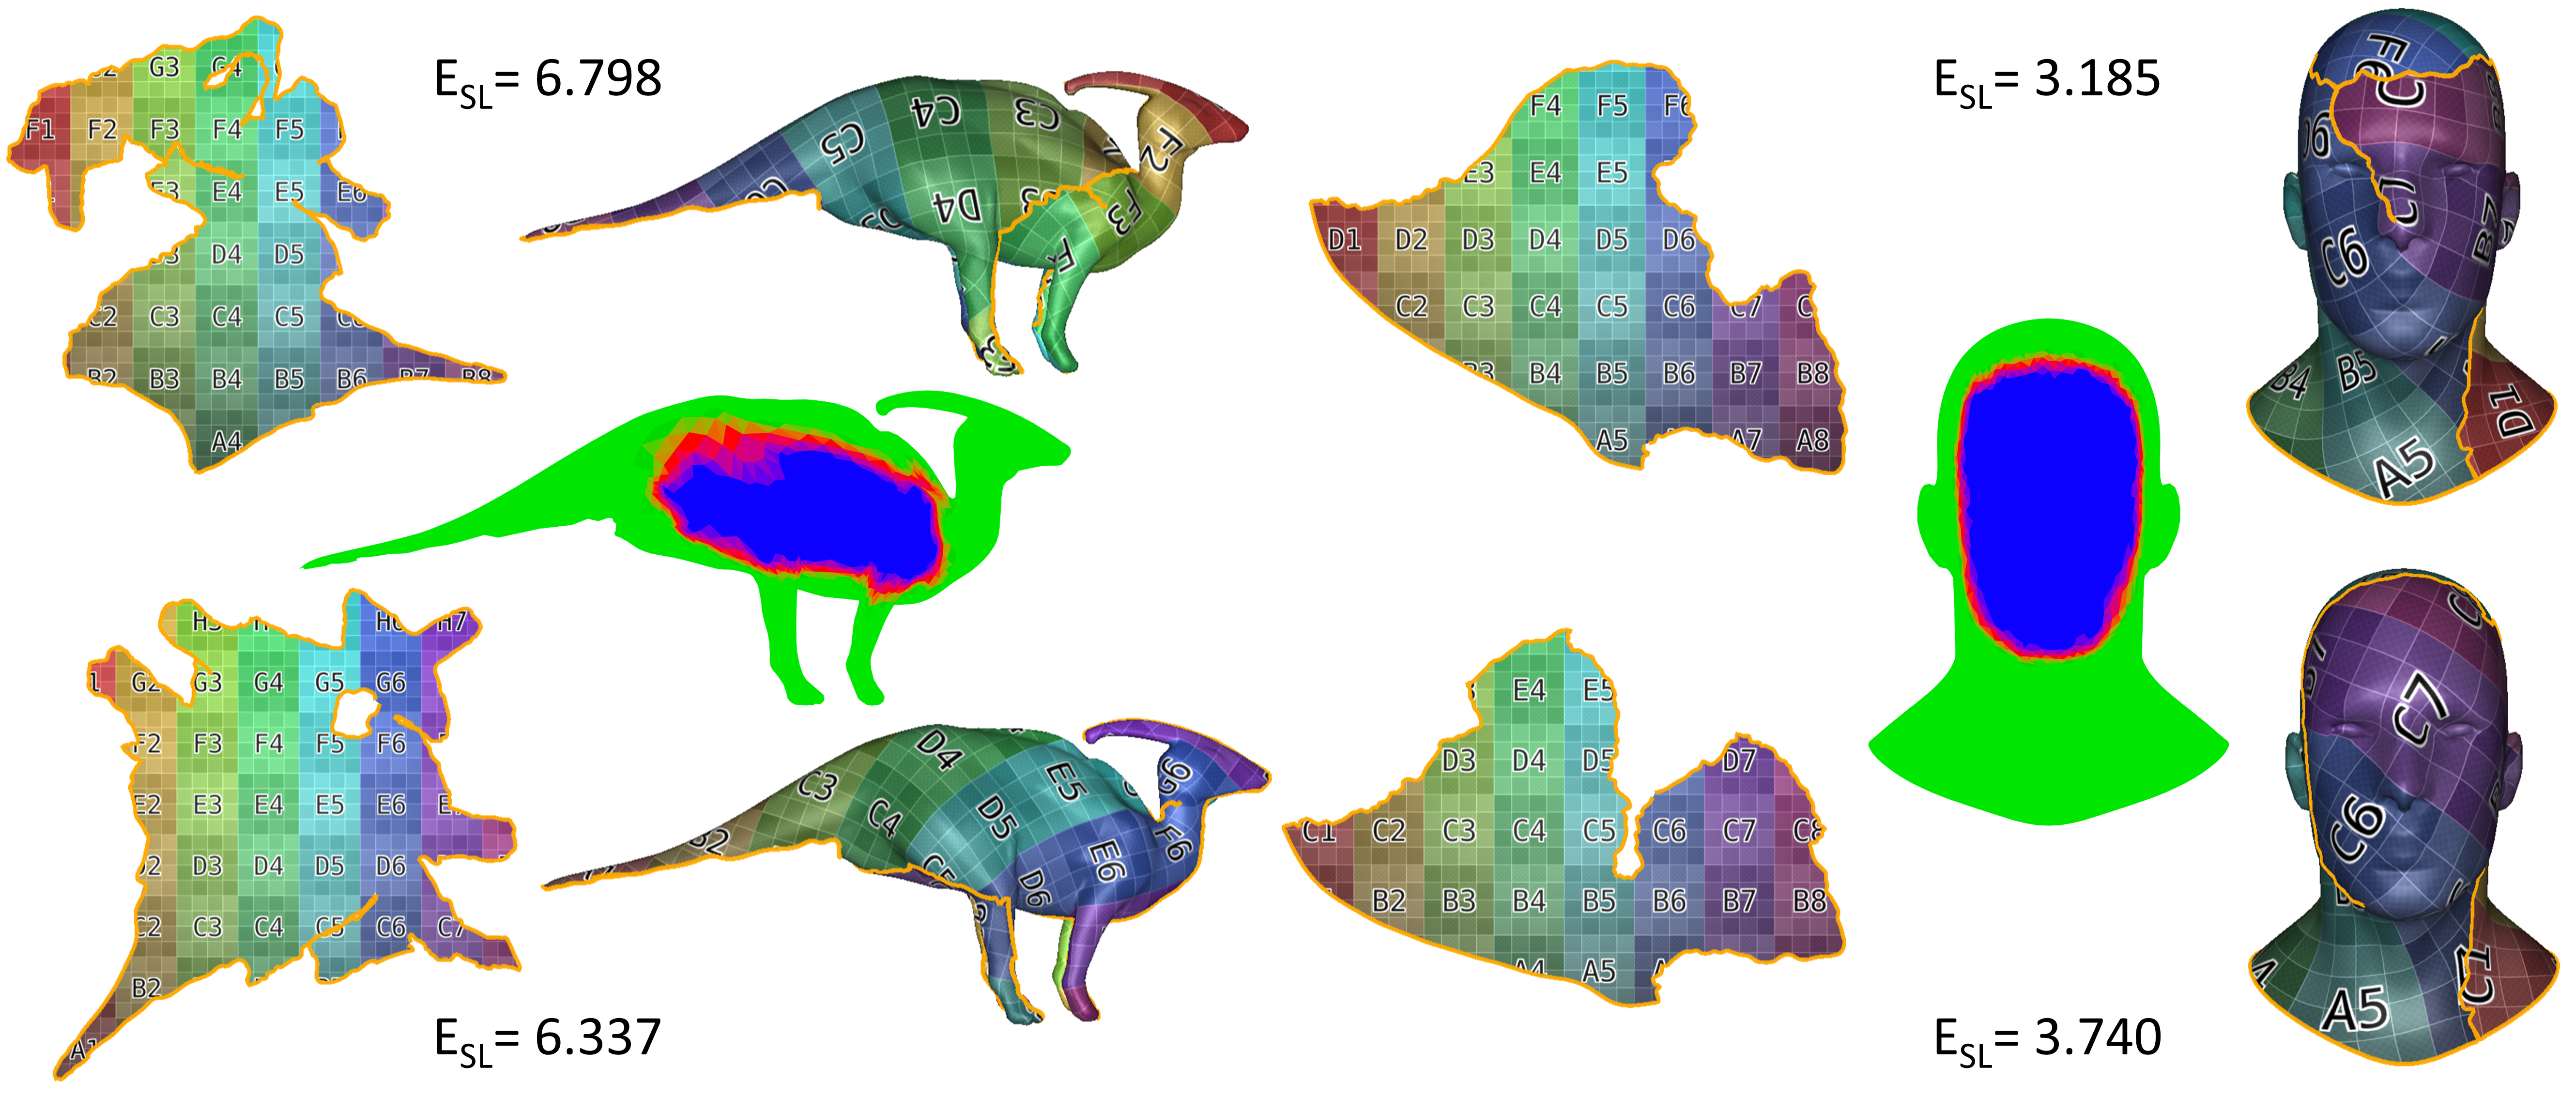
\includegraphics[width=\linewidth]{fig/regional_user.png}
\caption{Two examples with user-guided seam placement. The distortion bound is set to $b_d=4.1$ and we enforce bijectivity constraints in both cases. 
The fully automatic OptCut solution might place seams in salient regions (top), but the UV artist can paint ``do not cut here'' function (middle, blue), which will guide
the OptCut towards a better seam placement (bottom). Note that distortion and seam length is comparable in both cases. We happen to achieve shorter seams with additional user constraints for the dinosaur model since our method searches for a local optimum.}
\label{fig:regional_seam_placement}
\end{figure}

% \paragraph{Conformal Parameterization}
% Using a conformal energy~\cite{Hormann2000MIPS,Sheffer2005ABFPP} for $E_d$ will achieve joint seam placement and conformal parameterization. Figure~\ref{fig:conformal_vs_isometry} shows some results with $E_d = E_{ABForMIPS}$~\cite{} compared to results with $E_d = E_{d}$, where different seams are generated while our framework stays the same.

\paragraph{Alternative Cutting Strategy}
Our topology descent step leverages a small set of local topological operations to keep the framework simple and general. We also reduce the search complexity by filtering the candidates. Alternatively, one can use a richer set of more aggressive topological operations. For example, Geometry Images~\cite{Gu2002Geometry} leverage extrema-to-boundary cuts that connect the current boundary to the most distorted point (under current parameterization) using the shortest geodesic path. The advantage of this strategy is that it introduces more drastic topological updates at each iteration, potentially saving computational effort. We replace our topological search with this strategy (still terminating once $b_d$ is reached) and refer to the resulting variant of our method as EBCuts. As expected we found that the resulting approach is faster, but we found that it yields longer seams especially with tighter distortion bounds (Table~\ref{tb:comp_GI}) and for nearly-isometric UV maps where extremities are less prominent (Figure~\ref{fig:comp_GI}).
%\vova{We used notation $\mathcal{G}_T$ here, I don't think it appeared anywhere in the paper, so I removed it... we can define it earlier and bring it back if necessary...}

%The cutting strategy in the topology descent steps essentially build up the structure of the UV topology graph $\mathcal{G}_T$. By considering local topological operations, we built a dense graph connecting almost all the possible UV topologies and then reduce the search complexity by filtering. Alternatively, one can consider building $\mathcal{G}_T$ using only a sparse set of UV topologies and more aggressive topological operations, like the extremity-boundary (EBCuts) cut applied in Geometry Images~\cite{Gu2002Geometry}.


%We could alternatively apply EBCuts strategy in our framework without bijectivity constraints by simply alternating the cut with distortion minimization processes, and stop right after $b_d$ is reached. This variation of our method reaches identical distortion bounds with very similar seam length compared to our standard method, but is much faster since the EBCuts cut can be decided nearly instantly (Table~\ref{tb:comp_GI}). However, when we set smaller distortion bounds, the quality of the seams by EBCuts cut drops since extremities are not that obvious on a nearly isometric UV map (Figure~\ref{fig:comp_GI}).

\begin{table}[t]
\centering
\caption{Comparison between the standard OptCuts and using EBCuts cutting strategy in our framework, both without bijectivity constraints. We run the two methods on our benchmark and report statistics. EBCuts variant of our method is faster, but tends to produce longer seams.} 
\label{tb:comp_GI}
\begin{tabular}{|c|c|ccc|ccc|}
\hline
\multirow{2}{*}{$b_d$} & \multirow{2}{*}{strategy} & \multicolumn{3}{c|}{$E_{s}$} & \multicolumn{3}{c|}{time (s)} \\ \cline{3-8} 
                       &                         & avg      & min     & max      & avg       & min    & max      \\ \hline
\multirow{2}{*}{4.2}   & OptCuts                    & 3.819   & 0.080  & 14.545  & 87.0   & 0.3 & 417.8 \\
                       & EBCuts                & 3.868   & 0.159  & 14.929  & 13.0   & 0.1 & 72.1  \\ \hline
\multirow{2}{*}{4.1}   & OptCuts                    & 4.709   & 0.752  & 17.980  & 137.5  & 0.9 & 886.9 \\
                       & EBCuts                & 4.795   & 1.207  & 16.895  & 17.0   & 0.1 & 87.2  \\ \hline
\multirow{2}{*}{4.05}  & OptCuts                    & 6.142   & 0.277  & 21.566  & 213.2  & 3.9 & 1398.1   \\
                       & EBCuts                & 6.335   & 0.328  & 23.051  & 24.1   & 0.1 & 115.4 \\ \hline
\end{tabular}
\end{table}

\begin{figure}[t]
\centering
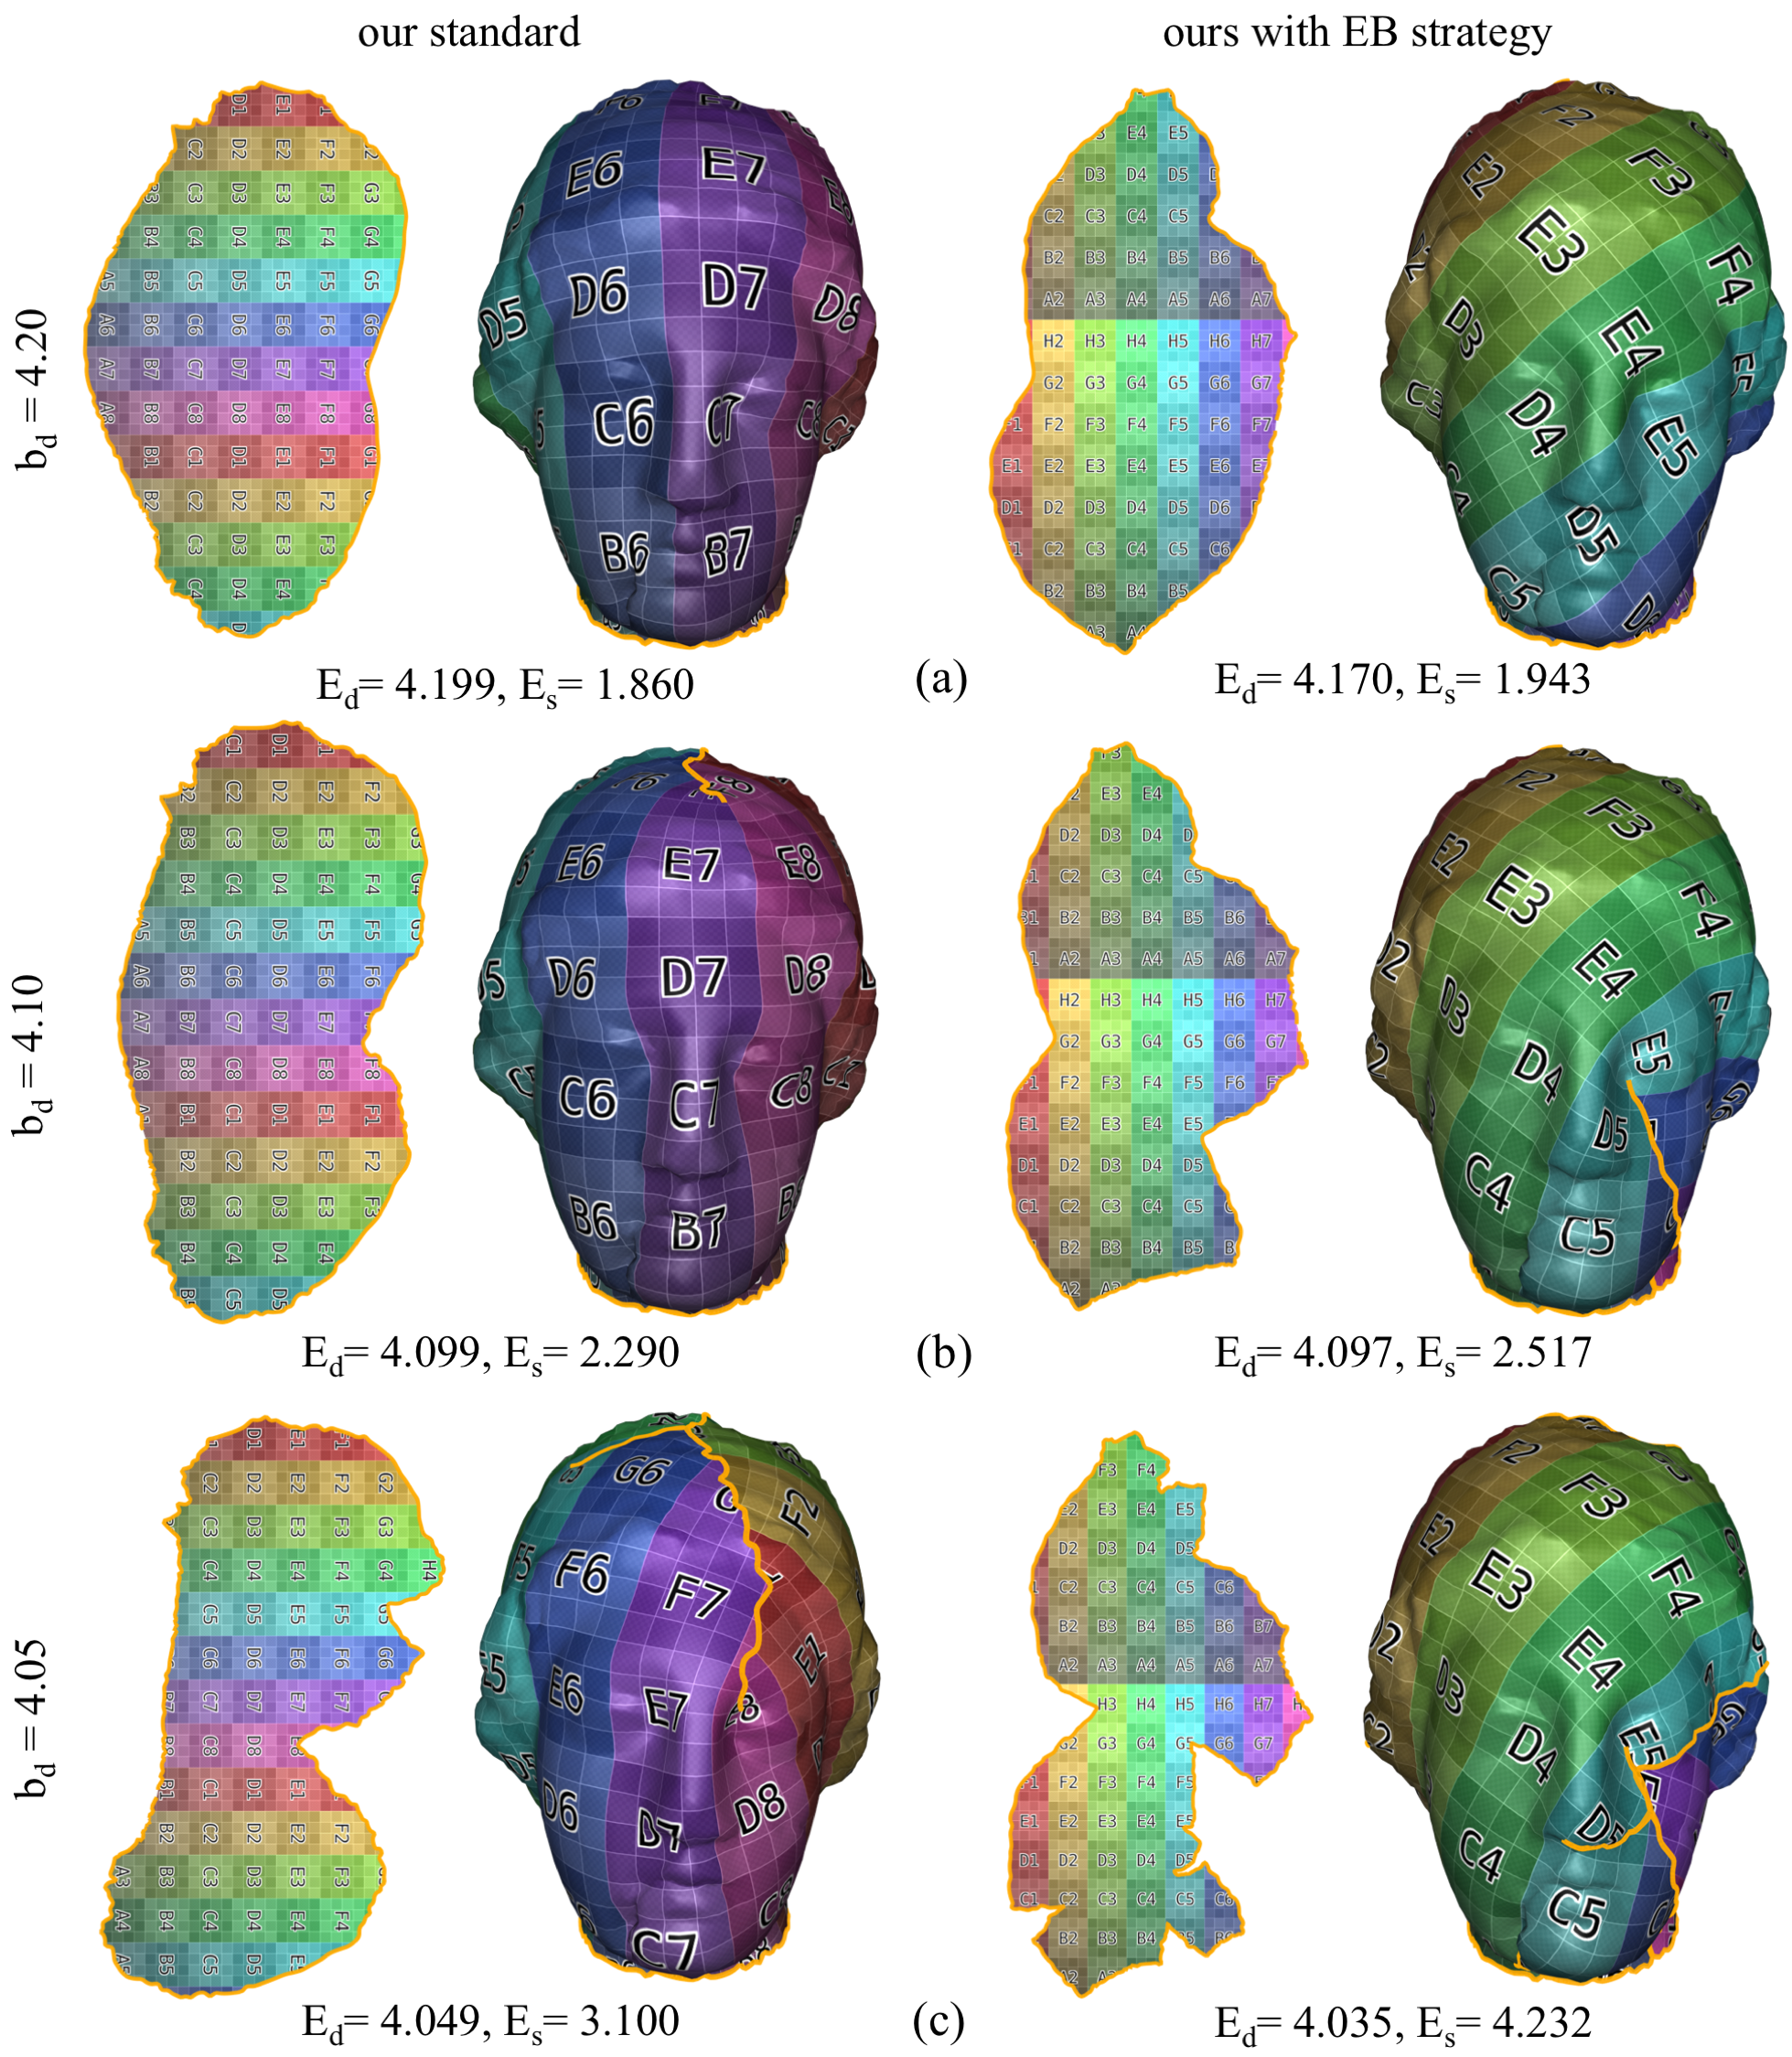
\includegraphics[width=0.8\linewidth]{fig/comp_GI.png}
\caption{Comparison between the standard OptCuts (left) and using EBCuts strategy in our framework (right), both without bijectivity constraints. EBCuts cutting strategy is very efficient in early stages (a, b), but it does not work well when the UV map gets closer to isometric where extremities are not very prominent (c).}
\label{fig:comp_GI}
\end{figure}
% also could be face_f10000, male_body_i_f10000, statue_4_i_f10000, statue_5_i_f10000, bimba_i_f10000

\paragraph{Warm Start}
Since our framework only provides local optima for a highly non-convex problem, initial conditions are relevant for the final result and computational cost. Several powerful topological heuristics have been used to provide a disk topology after cutting. %for the geometry optimization algorithm. 
We can consider any of these methods as a way to define an initialization for our approach. 

%Although we obtain high quality results given any initial embedding, the starting point does affect which local optimal point we will reach. Hence, it is meaningful to explore our method starting from initial seams with global observations. This will also benefit practical scenarios for improving preliminary UV maps while stay close to it.

As first example, we take the seams produced by our method with the EBCuts strategy and construct the initial embedding using our standard approach of Tutte's parameterization followed by distortion minimization. We can improve the seam quality while respecting the distortion bound by leveraging our local topological search which enables us to close unnecessary cuts by merging. Even with the bijectivity constraints, we still achieve shorter seam length (Figure~\ref{fig:comp_GI_outputAsInit}).

\begin{figure}[t]
\centering
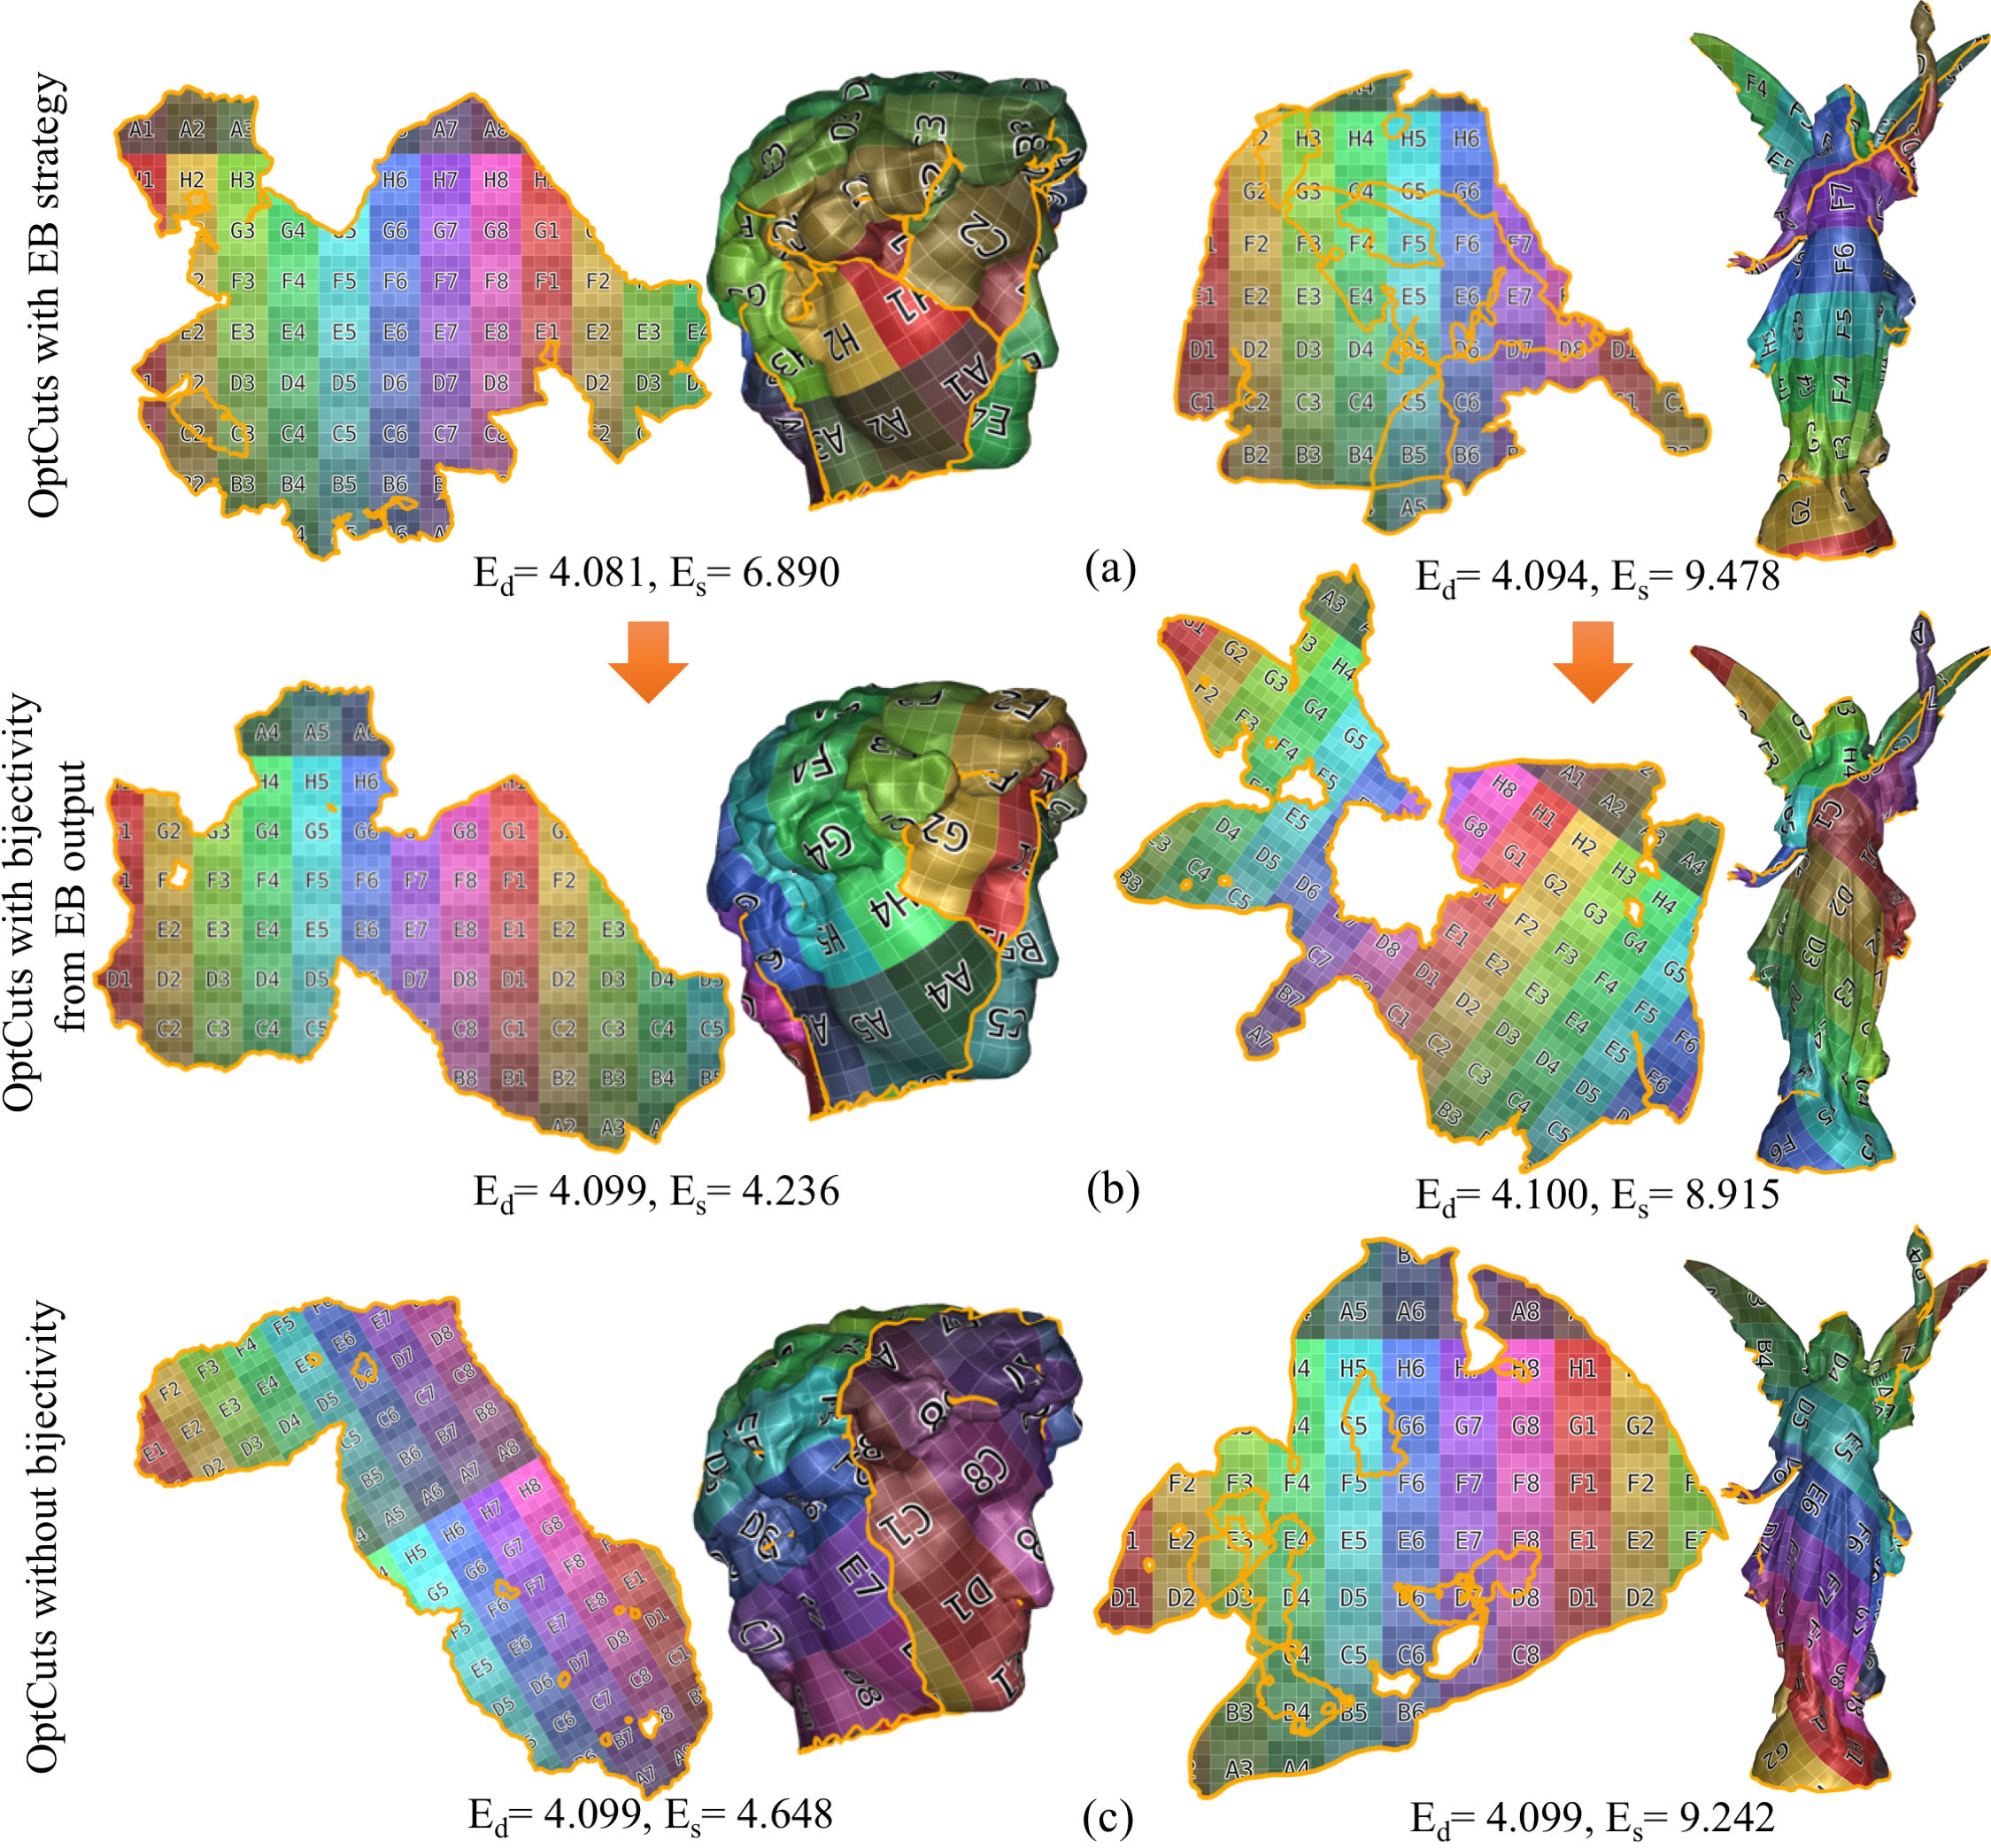
\includegraphics[width=\linewidth]{fig/comp_GI_outputAsInit.png}
\caption{We use the seams produced by our framework with EBCuts strategy at $b_d = 4.1$  initial UV map (a). We ran our OptCuts framework to improve the seam quality, reaching a locally optimal seam configuration under the given distortion bound even with bijectivity constraints (b). This seam length is also shorter than results obtained by standard OptCuts without bijectivity (c).}
\label{fig:comp_GI_outputAsInit}
\end{figure}
% also could be bimba, bunny

The second option we explore is Seamster~\cite{Sheffer2002Seamster}, a classic seam cutting strategy that detects local curvature extrema and connects them with a minimal spanning tree.  This approach can be sensitive to the user-set parameters such as size of surface regions for computing local extrema, which is a shape-dependent parameter that might require tuning. In this experiment, however, we pick two models that have been successfully cut with Seamster (a cow and a triceratops) and use our standard approach to produce the initial embedding, i.e., Tutte's embedding followed by minimizing $E_{d}$ with bijectvitiy constraints (Figure~\ref{fig:comp_Seamster}a). We use the resulting distortion as the upper bound and run the full OptCuts framework on the result. As demonstrated in Figure~\ref{fig:comp_Seamster}b, we achieve shorter seam length while maintaining the distortion bound and bijectivity. This seam length is also shorter than running our standard method without bijectivity from standard initialization (Figure~\ref{fig:comp_Seamster}c).

%With Seamster's best output seams on the cow and triceraptop model, we obtain UV maps by minimizing $E_{d}$ with bijectivity constraints (Figure~\ref{fig:comp_Seamster}a), and use them for warm start, setting their distortions as the upper bounds. As demonstrated in Figure~\ref{fig:comp_Seamster}b, we achieve shorter seam length while maintaining the distortion bound and bijectivity. This seam length is also shorter than running our standard method without bijectivity from standard initialization (Figure~\ref{fig:comp_Seamster}c).

\begin{figure}[t]
\centering
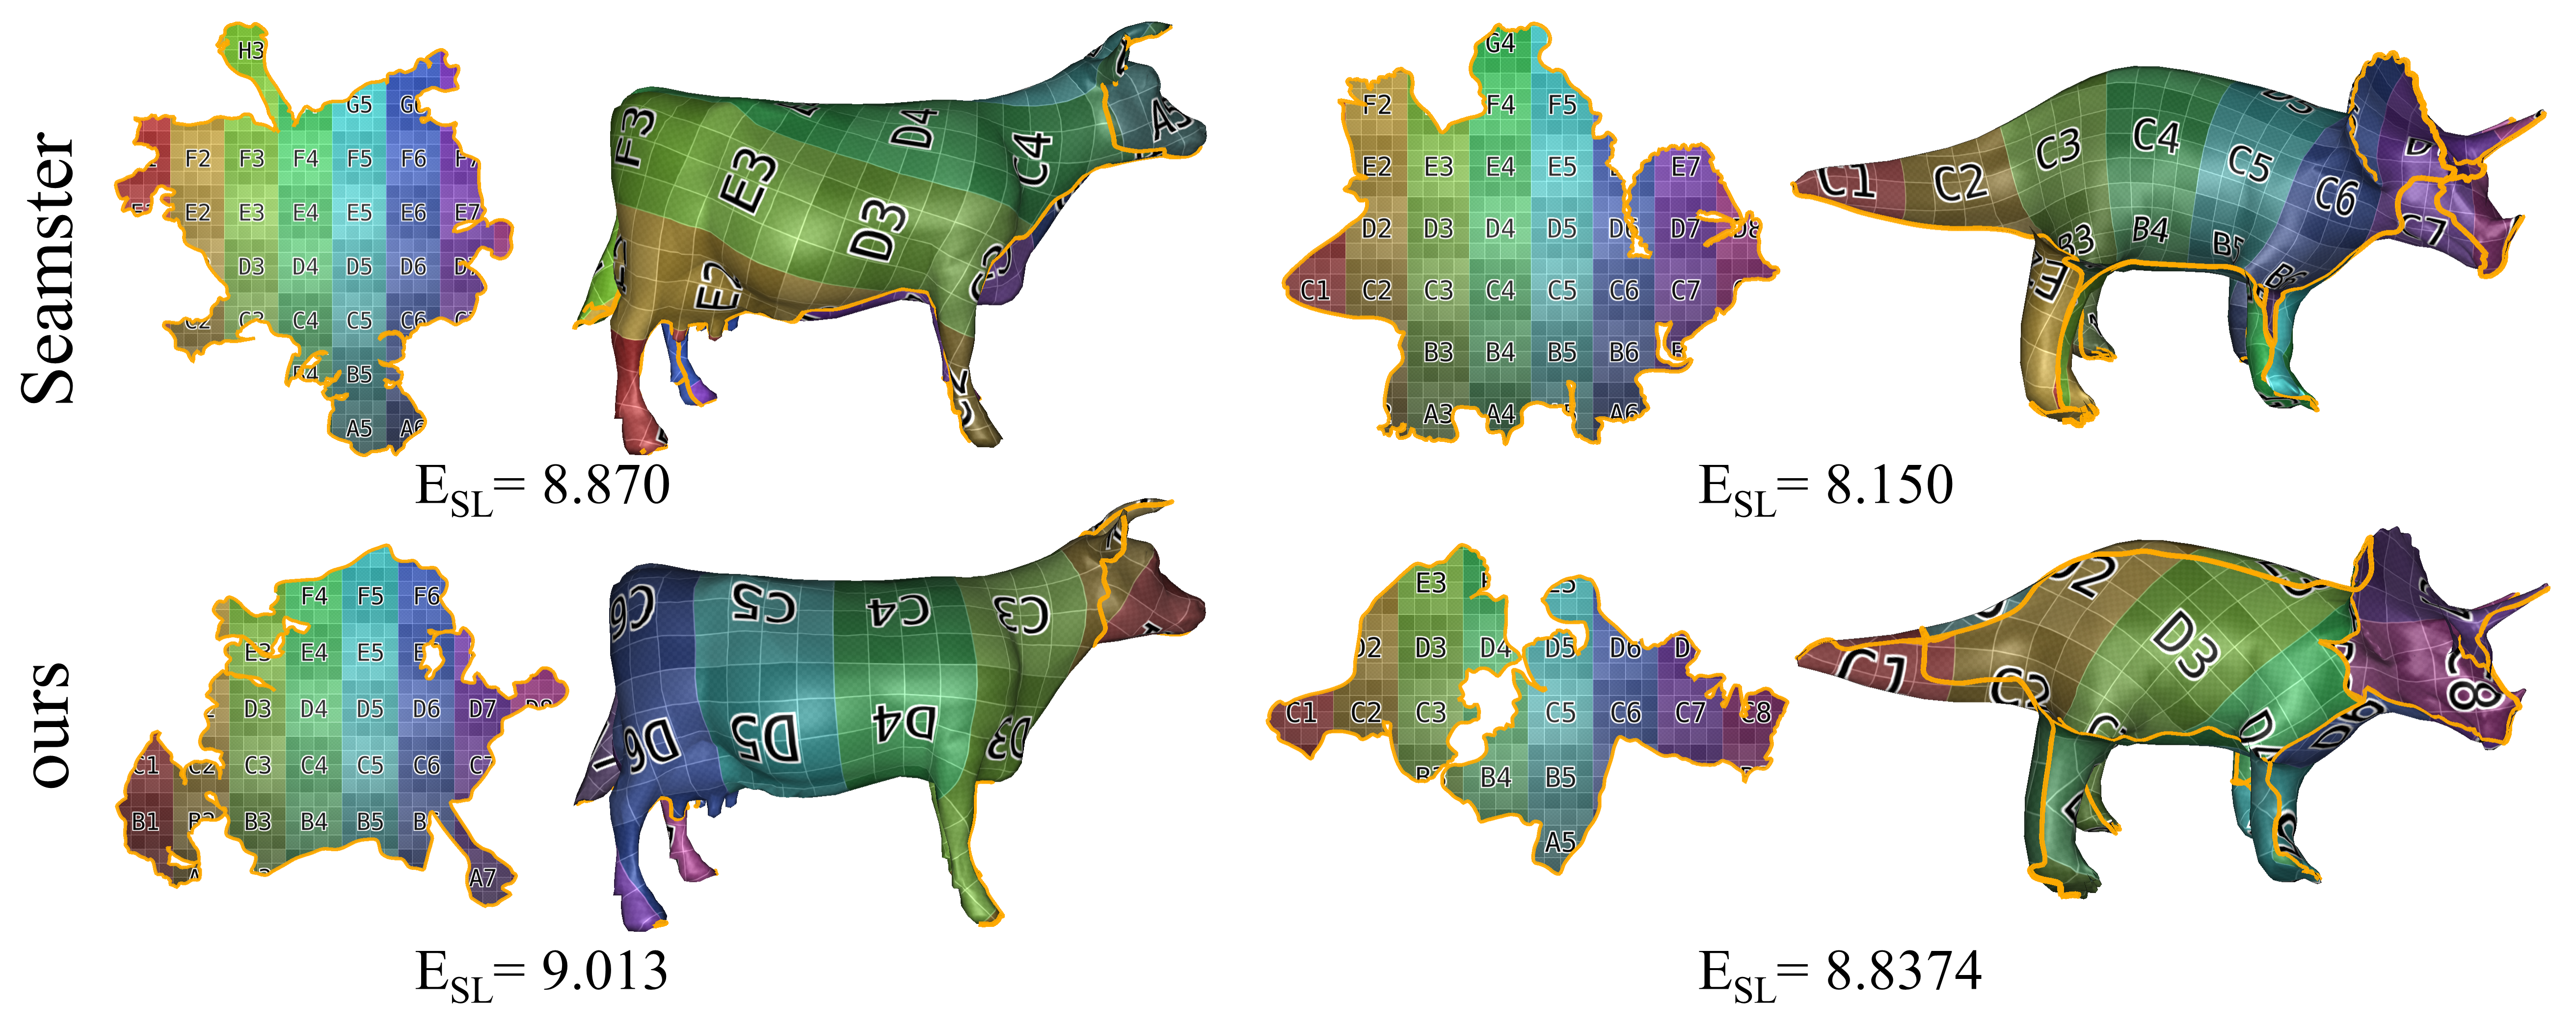
\includegraphics[width=\linewidth]{fig/comp_Seamster.png}
\caption{Starting from UV maps obtained by using Seamster's best output seams (a), we improve seam quality, reaching a locally optimal seam configuration while maintaining the distortion and bijectivity (b). This seam length is also shorter than running standard OptCuts without bijectivity from standard initialization (c).}
\label{fig:comp_Seamster}
\end{figure}

%For Seamster, user need to set the size of local regions for measuring extremity, which is a mesh and shape dependent parameter that requires fine tuning. Even OptCuts with standard initialization achieves similar seam length without any user assistance.



\section{Conclusions and Future Works}

take advantage of basic SIMD type of parallelism for accelerating query and improving results' quality by directly evaluating $f_v$ for neighbors and track multiple branches, very useful for practical implementations

if the user won't mind getting a slightly different triangulation, we could also create fractures in the interior of an element and locally remesh the stencil

start and solve in 3D by reducing curvature so that the need for locally injective initial embedding in parameterization problems could be eliminated, and the result is only "biased" by it's 3D shape, which is the most reasonable bias

try conformal energy like MIPS

bijectivity, seamless, and other augmentation of continuous energy?

handle user preferences on seam placement

seam smoothness, patch related discrete energy augmentation?

\section{Acknowledgements}

\bibliographystyle{ACM-Reference-Format}
\bibliography{OptCuts} 

\end{document}
